%%%%%%%%%%%%%%%%%%%%%%% file template.tex %%%%%%%%%%%%%%%%%%%%%%%%%
%
% This is a general template file for the LaTeX package SVJour3
% for Springer journals.          Springer Heidelberg 2010/09/16
%
% Copy it to a new file with a new name and use it as the basis
% for your article. Delete % signs as needed.
%
% This template includes a few options for different layouts and
% content for various journals. Please consult a previous issue of
% your journal as needed.
%
%%%%%%%%%%%%%%%%%%%%%%%%%%%%%%%%%%%%%%%%%%%%%%%%%%%%%%%%%%%%%%%%%%%
%
%\documentclass{svjour3}                     % onecolumn (standard format)
%\documentclass[smallcondensed]{svjour3}     % onecolumn (ditto)
\documentclass[smallextended]{svjour3}       % onecolumn (second format)
%\documentclass[twocolumn]{svjour3}          % twocolumn
%
\smartqed  % flush right qed marks, e.g. at end of proof
%
\usepackage{graphicx}
\usepackage{amssymb}
\usepackage{amsmath}
\usepackage{hyperref}
%\usepackage{academicons}
%\RequirePackage[colorlinks,citecolor=blue,urlcolor=blue]{hyperref}
%
% \usepackage{mathptmx}      % use Times fonts if available on your TeX system
%
% insert here the call for the packages your document requires
%\usepackage{latexsym}
% etc.
%
% please place your own definitions here and don't use \def but
% \newcommand{}{}
%
% Insert the name of "your journal" with
\journalname{Optimization Letters}
%
\begin{document}

\title{A Computationally Efficient Approach for Solving Lexicographic Multicriteria Optimization Problems\thanks{This research was supported by the Russian Science Foundation, project No 16-11-10150 ``Novel efficient methods and software tools for time-consuming decision making problems using supercomputers of superior performance''.}
}

\titlerunning{Efficient Approach for Solving Multicriteria Optimization Problems}        % if too long for running head

\author{Victor Gergel %\href{https://orcid.org/0000-0002-4013-2329}{
\includegraphics{ORCID.png}}
%\orcidID{0000-0002-4013-2329} 
\and
Evgeniy Kozinov
%\orcidID{0000-0001-6776-0096} 
\and
Konstantin Barkalov
%\orcidID{0000-0001-5273-2471}
}

%\authorrunning{Short form of author list} % if too long for running head

\institute{               
V. Gergel \at
Lobachevsky State University of Nizhni Novgorod, Nizhni Novgorod, Russia \\
\email{gergel@unn.ru} 
\and
E. Kozinov \at
Lobachevsky State University of Nizhni Novgorod, Nizhni Novgorod, Russia \\
\email{evgeny.kozinov@itmm.unn.ru} 
\and
K. Barkalov \at
Lobachevsky State University of Nizhni Novgorod, Nizhni Novgorod, Russia \\
\email{konstantin.barkalov@itmm.unn.ru}
}

\date{Received: date / Accepted: date}
% The correct dates will be entered by the editor

\maketitle

\begin{abstract}
This paper proposes a computationally efficient approach for solving complex lexicographic multicriteria optimization problems in which efficiency criteria can be multiextremal and computing the values of criteria can be time-consuming. It is also assumed that in the course of calculations, how problems are formulated may change and consequently, solving dynamically defined sets of multicriteria optimization problems may become necessary. The proposed approach is based on reducing multidimensional problems to one-dimensional global optimization problems, utilizing efficient global search algorithms, and reusing the search information obtained in the process of calculations. Results of computational experiments demonstrate that the proposed approach can significantly reduce the computational complexity of solving multicriteria optimization problems.
\keywords{Multicriteria optimization \and Lexicographic ordering \and Global optimization \and Dimensionality reduction \and Search information \and Computational complexity}
\end{abstract}

\section{Introduction}
\label{sec:1}

Multicriteria optimization (MCO) problems are among the most common statements used to address decision-making problems and are widely found in applications. Multicriteria optimization is an area of vigorous scientific research, and during this time a large number of efficient methods of multicriteria optimization have been proposed and many practical problems have been solved (see, e.g., monographs \cite{c1,c2,c3,c4}) and reviews of scientific and practical results in this field \cite{c6,c7,c8,c9}.

A key feature of MCO problems is the absence, in most cases, of a single decision which would best fulfill all efficiency criteria, due to possible inconsistencies. As a result, solving MCO problems usually requires finding several compromise (efficient and non-dominated) decisions that cannot be improved without damaging the effectiveness of some efficiency criteria in the MCO problem.

Among the approaches which have been developed for solving MCO problems, lexicographic optimization methods can be singled out, when some ordering of criteria by importance is implemented and optimization is carried out based on their ordering \cite{c3}. Iterative methods represent another approach \cite{c6,c10}, when the decision maker is actively involved in the process of selecting decisions. An actively appropriated approach consists in developing and applying evolutionary algorithms based on the simulation of certain natural phenomena to solve MCO problems \cite{c10,c11,c12,c13}. Among the widely used endeavors in solving MCO problems is the scalarization approach, which applies methods involving the convolution of criteria to a single scalar criterion (see, e.g. \cite{c2,c14}).

This work is devoted to solving lexicographic multicriteria optimization (MCOlex) problems that arise when designing complex technical objects and systems. In such applications, efficiency criteria may have a complex multiextremal form, and calculating criteria values may require large amounts of computations. In such conditions, finding even one efficient decision requires significant calculations, while determining several (or a whole set) of efficient decisions becomes an issue of great computational complexity.

The properties listed above highlight a key feature of the MCOlex problems   high computational complexity. One promising attempt to solve such problems is using the model-based approach, when, after a small number of calculations determining the values of time-consuming criteria and, fast-computable approximating functions are constructed \cite{c15,c16}. This approach is quite efficient; however, it is difficult to construct good approximations given the multiextremal behavior of efficiency criteria.

This paper proposes a solution to the time-consuming class of MCOlex problems by using an approach based on the following main points. First of all, the problem is reduced to solving a sequence of global optimization problems with nonlinear constraints (GCO) \cite{c2,c14}. Then, efficient global search algorithms developed in the framework of the information-statistical theory of multiextremal optimization are applied for solving the GCO problems \cite{c17,c18}. And finally, the search information obtained in the process of solving the MCOlex problem is fully utilized. In general, the developed approach allows us to significantly reduce the amount of executed computations, up to just a few iterations when searching for new efficient decisions.

The further structure of the paper is as follows. Section \ref{sec:2} presents a new class of optimization problems -- multistage lexicographic multicriteria optimization (MMCOlex) problems -- whose solution is reduced to solving a sequence of global optimization problems with nonlinear constraints. Section \ref{sec:3} presents the basics of the approach that has been developed: reducing multidimensional MCOlex problems to one-dimensional global optimization problems, applying efficient global search algorithms developed in the framework of the information-statistical theory of multiextremal optimization, and reusing the search information obtained in the process of calculations. Section \ref{sec:4} contains the results of numerical experiments. The paper concludes by discussing the results that were obtained and suggests some main directions for further research.

\section{Problem statement}
\label{sec:2}

The multicriteria (or vector) optimization (MCO) problem can be defined as follows:
\begin{equation}\label{eq:1}
f(y) = (f_1(y), f_2(y), \dots , f_s(y)) \to min, \; y \in D,
\end{equation}
where $f(y) = (f_1(y), f_2(y), \dots , f_s(y))$ is the vector efficiency criterion, $y = (y_1, y_2, \dots , y_N)$ is the vector of variable parameters, and $N$ is the dimension of the multicriteria optimization problem to be solved. The search domain $D$ defines the set of possible parameter values and is usually an $N$-dimensional hypercube
\begin{equation}\label{eq:2}
D  = \{ y\in R^N: a_i \leq y_i \leq b_i, \; 1 \leq i \leq N \}
\end{equation}
for the given boundary vectors $a$ and $b$.

Without a loss of generality, it is assumed that the values of the efficiency criteria are not negative and their decrease corresponds to an increase in the effectiveness of the considered decisions $y \in D$. Problem (\ref{eq:1}) is considered in relation to the most difficult decision-making problems in which the efficiency criteria $f_i(y)$, $1 \leq i \leq s$, can be significantly multiextremal, and the procedures for calculating the values of efficiency criteria at points of the search domain $y \in D$ can be computationally expensive. It is also assumed that the criteria $f_i(y)$, $1 \leq i \leq s$, satisfy the Lipschitz condition
\begin{equation}\label{eq:2l}
|f_i (y')-f_i (y'')| \leq L_i \|y'-y''\|, \; y',y''\in D,\; 1 \leq i \leq s,
\end{equation}
where $L_i$ is the Lipschitz constants for the function $f_i(y)$, $1 \leq i \leq s$, and $\|*\|$ denotes the Euclidean norm in $R^N$. Fulfillment of the Lipschitz condition means that for small variations of the decision $y \in D$, corresponding changes in the values of the criteria $f_i(y)$, $1 \leq i \leq s$, are limited.

In problem (\ref{eq:1}), the efficiency criteria are usually contradictory and there is no decision $y \in D$, that would provide the best (smallest) values for all criteria at the same time, i.e.
\begin{equation}\label{eq:3}
\nexists y^*\in D: f_i(y^*) = \min_{y \in D} {f_i (y)} , 1 \leq i \leq s.
\end{equation}

If the relation (\ref{eq:3}) is valid when solving the MCO problem, then decisions $\widetilde{y}^* \in D$ can be determined, at which the values of the criteria cannot be improved without deterioration of the values of some criteria $f_i(y)$, $1 \leq i \leq s$, that is
\begin{equation}\label{eq:4}
\nexists y'\in D: (f_i(y') \leq f_i(\widetilde{y}^*)), 1 \leq i \leq s, (\exists j : f_j(y') < f_j(\widetilde{y}^*)).
\end{equation}

Such non-improvable decisions are called Pareto \textit{efficient} or \textit{optimal}.

The Pareto set $P(f,D)$ of all efficient decisions can be quite large, which makes it difficult for the decision maker to analyze. A possible way to reduce the number of efficient decisions under consideration is to assume that the effectiveness criteria are ordered in terms of importance, which is often the case in practical applications.

Without a loss of generality, we will further assume that the criteria $f_i(y)$, $1 \leq i \leq s$, are ordered in importance according to their enumeration in (\ref{eq:1}). The ordering of the criteria determines the relative linear order in the search domain $D$, that is
\begin{equation}\label{eq:4d}
y' \prec y'' \Leftrightarrow \exists i, 1 \leq i \leq s: (f_i(y')<f_i(y'')) \wedge [ \forall j, 1 \leq j <i \Rightarrow (f_j(y')=f_j(y'')) ].
\end{equation}

As a result, problem (\ref{eq:1}) is reduced to the lexicographic multicriteria optimization problem (MCOlex)
\begin{equation}\label{eq:5}
f(y) = (f_1(y), f_2(y), \dots , f_s(y)) \to min_{lex},  y \in D,
\end{equation}
the solution of which is carried out in stages: initially, the first (most important) criterion is optimized; next, if the solution is not the only one, then the second criterion is optimized on the set of solutions of the first stage, and so on.
\begin{equation}\label{eq:6}
D_1=Arg \min_{y \in D}{f_1(y)},\dots, D_i=Arg \min_{y \in D_{i-1}}{f_i(y)},1 \leq i \leq s,D_0=D,
\end{equation}
where \textit{Arg} means the set of all decisions that achieve the minimum value of the optimized criterion. It should be noted that the sequence of steps in (\ref{eq:6}) may not be fully completed if at some stage $l$, $1 \leq l \leq s$, the set $D_l$ degenerates and contains only a single decision $y \in D$.

The set of efficient decisions $P_{lex}(f,D)$ obtained as a result of (\ref{eq:6}) is a subset of the Pareto domain $P(f,D)$ and can contain from one to several decisions $\widetilde{y}^* \in D$ in the case that the minimum value of the last criterion $f_s(y)$ is achieved at several points in the search domain $D$. Such a sharp reduction in the set of the efficient decisions being considered may be undesirable. Expanding the set of $P_{lex}(f,D)$ decisions can be achieved through somewhat weakening the ``strict'' lexicographic order and by allowing, at each stage of the computational scheme (\ref{eq:6}), the choice of decisions in a certain neighborhood of the minimum values of the optimized criterion, that is
\begin{equation}\label{eq:7}
\begin{matrix}
f^*_1 =\min_{y \in D}{f_1(y)},  \\
f^*_i =\min_{y \in D}{f_i(y)},  f_j(y) \leq f^*_j + \delta_j, 1 \leq j < i, 1 < i \leq s, \\
P_{lex}^\delta(f,\delta,D) = Arg \min_{y \in D}{f_s(y)},f_j(y) \leq f^*_j + \delta_j, 1 \leq j < i, 1 < i \leq s.
\end{matrix}
\end{equation}

This approach is also widely known as the method of successive concessions (MSC) \cite{c3,c4,c5}. The choice of feasible concessions $\delta_i$, $1 \leq i < s$, in the computational scheme (\ref{eq:7}) allows one to obtain any efficient decision $\widetilde{y}^* \in P_{lex}(f,D)$ and take into account the peculiarities of the MCOlex problem being solved. At the same time, this approach makes it necessary, at each stage of scheme (\ref{eq:7}), to solve more complex global optimization problems with nonlinear constraints.

It should also be noted that during the calculation process, it may be necessary to change the selected values of the feasible concessions $\delta_i$, $1 \leq i < s$; the concessions may be quite rigid or, conversely, excessively large. In general, one may need to change the order of importance in efficiency criteria. Such assumptions necessitate a more general formulation of how to solve the MCOlex problem and to provide possible solutions to many problems of the form (\ref{eq:7})
\begin{equation}\label{eq:8}
\mathbb{P}_t=\{ P_1,P_2,\dots,P_t\},
\end{equation}
which can be changed dynamically during calculations by adding new or deleting existing multicriteria optimization problems. In general, such an approach defines a new class of optimization problems: multistage lexicographic multicriteria optimization problems (MMCOlex).

\section{The Approach: Key Ideas and Methods}
\label{sec:3}

The extended formulation of lexicographic multicriteria optimization problems (\ref{eq:7})--(\ref{eq:8}) involves multiple solutions of multiextremal optimization problems with nonlinear constraints. Problems of this type are computationally time-consuming and subject to the ``curse of dimensionality'' -- computational complexity increases exponentially with increasing dimensionality. The proposed approach for solving such problems is based on three key ideas:
\begin{itemize}
  \item Reduction of multidimensional problems of multiextremal optimization to problems of one-dimensional global search by using mappings based on Peano curves;
  \item Using the index method of global optimization, which allows solving optimization problems with constraints without using penalty functions;
  \item Repeated use of search information obtained in the process of computing, for solving multiple global optimization problems.
\end{itemize}

\subsection{Dimension reduction of multidimensional multicriteria optimization problems}

The search for numerical estimates of globally optimal points involves the construction of grids covering the search domain $D$ (see, e.g., \cite{c17,c18,c19,c20,c21,c22,c23,c24,c25}). This key feature of global optimization problems leads to the ``curse of dimensionality'', where the computational complexity of constructing coverage increases exponentially as the dimensions of optimization problems are enlarged. Significantly reduced complexity can be achieved by using heterogeneous grids that are denser only in the vicinity of globally optimal points. Such heterogeneous coverage of the search domain $D$ can be constructed adaptively in the following manner: when choosing points for the next iterations, the global search is performed taking into account all the available search information (points of previous search iterations and values of the optimized function at these points), that is
\begin{equation}\label{eq:9}
y^{k+1}=G_k(\omega_k), \omega_k=\{(y^i,f^i=f(y^i)): 1 \leq i \leq k \},
\end{equation}
where $k$ is the number of the global search iterations being performed, $G_k$ is the decisive rule of the applied global search algorithm, according to which the point $y^{k+1}$ of the next iteration is selected, and $\omega_k$ is the search information available at the $k$ step of the global search.

Adaptive selection of points $y^{k+1} \in D$ at the iterations of the global search involves the analysis of volumetric multidimensional search information $\omega_k$ $(k \gg 1)$, which determines the high computational complexity of the decisive rules $G_k$, $k=1,2,\dots$ of global search algorithms. This computational complexity can be significantly simplified by reducing the optimization problems to be solved using Peano \textit{space-filling curves} or \textit{evolvents} $y(x)$, that uniquely and continuously map the interval $[0,1]$ to an $N$-dimensional hypercube $D$ (see, e.g., \cite{c17,c18,c23}). As a result of this reduction, the initial multidimensional multicriteria optimization problem (\ref{eq:5}) is reduced to a one-dimensional problem:
\begin{equation}\label{eq:10}
f(y(x)) = (f_1(y(x)), f_2(y(x)), \dots , f_s(y(x)) \to min_{leq},  x \in [0,1].
\end{equation}

It should be noted that the one-dimensional functions obtained as a result of the reduction satisfy the uniform H\"older condition (see \cite{c17,c18}), that is
\begin{equation}\label{eq:11}
|f_i (y(x'))-f_i (y(x''))| \leq H_i \|x'-x''\|, \; x',x''\in [0,1],\; 1 \leq i \leq s,
\end{equation}
where the constants $H_i$ are determined by the ratio $H_i=2L_i\sqrt{N+3}$, $1 \leq i \leq m$, $L_i$ are the Lipschitz constants from (\ref{eq:2l}), and $N$ is the dimension of the optimization problem (\ref{eq:1}).

Using dimension reduction the search information $\omega_k$ can be converted from (\ref{eq:9}) to the form
\begin{equation}\label{eq:12}
A_k=\{(x_i, y(x_i), f_i=f(y(x_i))): 1 \leq i \leq k \},
\end{equation}
in which, in addition to the reduced representation, the data is arranged in ascending order\footnote{Data ordering is reflected by using a subscript.} of points $x_i$, $1 \leq i \leq k$, that is
\begin{equation}
x_1 < x_2 < \dots < x_k	
\end{equation}
for a more efficient execution of global search algorithms.

Dimension reduction using Peano curves is widely used in the development of efficient global search algorithms in the framework of the information-statistical theory of multiextremal optimization \cite{c17,c18,c23,c26,c27}. Numerical methods for constructing approximations of Peano curves (\textit{evolvents}) with a given accuracy are considered in \cite{c17,c18}.

\subsection{An efficient method for solving global optimization problems with 
nonlinear constraints}

The problems solved in the framework of the computational scheme (\ref{eq:7}) are one-dimensional global optimization problems with nonlinear constraints
\begin{equation}\label{eq:13}
\min{\{\varphi(x):g_i(x)\leq 0, \; 1 \leq i \leq m,\; x\in \Delta=[0,1]\}}
\end{equation}
(the notation $g_{m+1}(x) = \varphi(x)$ will also be used later).

The presence of nonlinear constraints significantly complicates the complexity of solving global optimization problems; the resulting solutions must belong to a feasible domain
\begin{equation}\label{eq:14}
\Delta_g  = \{ x\in \Delta=[0,1]:g_i(x)\leq 0,   1 \leq i \leq m \}.
\end{equation}

To reduce the complexity of solving optimization problems with constraints, simpler cases are often highlighted; for example, problems with linear or quadratic constraints are selected. Various methods of approximating complex constraints with the aid of simpler forms (linear, convex, etc.) are widely used. However, the penalty function method is most commonly used, when calculating in an unfeasible region $\Delta \setminus \Delta_g$, some ``penalty'' is added to the values of the minimized function. But the penalty function method often involves repeatedly solving the optimization problem to determine a sufficient value of the penalty coefficient. More complete information on methods for solving optimization problems with constraints can be obtained, for example, in monographs \cite{c18,c26,c27}.

The proposed approach is based on the original method of separate accounting for constraints developed in the framework of the information-statistical theory of multiextremal optimization \cite{c18}. The key idea of the approach consists in constructing a certain integral objective function without constraints, the solution of which also provides a solution to the initial constrained optimization problem (\ref{eq:13}); a more detailed presentation of this method is given below.

We apply a sequential scheme to obtain the constraint values $g_i(y(x)) \leq 0$, $1 \leq i \leq m$, and the minimized function $\varphi(x)$, according to which the constraint values are calculated strictly in the order of their numbers, and the calculations immediately stop when the first violated constraint is detected (the partial computability scheme). The number of constraints in which the values were calculated will be indicated below as the index $\nu=\nu(x)$, that is
\begin{equation}\label{eq:15}
\nu(x) : g_\nu(x)>0, g_j(x)\leq 0, 1 \leq j\leq \nu - 1, 1\leq \nu = \nu(x) \leq m
\end{equation}
 (when all the constraints are satisfied, $\nu=m+1$ is assumed). Introducing the index concept allows us to determine the integrated function for the problem (\ref{eq:13}) (see Fig. \ref{fig:1})
\begin{equation}\label{eq:16}
F(x)=g_\nu(x), \nu=\nu(x),
\end{equation}
defined and computable everywhere in $[0,1]$. Its value at the point $x\in [0,1]$ is either the value of the left side of the constraint violated at this point (the case when $\nu \leq m$), or the value of the minimized function (the case when $\nu = m + 1$). The process of calculating the value of $F(x)$, $x\in [0,1]$, is completed either as a result of establishing the inequality $g_j(x)>0$, or as a result of reaching the value $\nu(x)=m+1$ (below, this procedure is called a \textit{trial}).

\begin{figure}
  \centering
  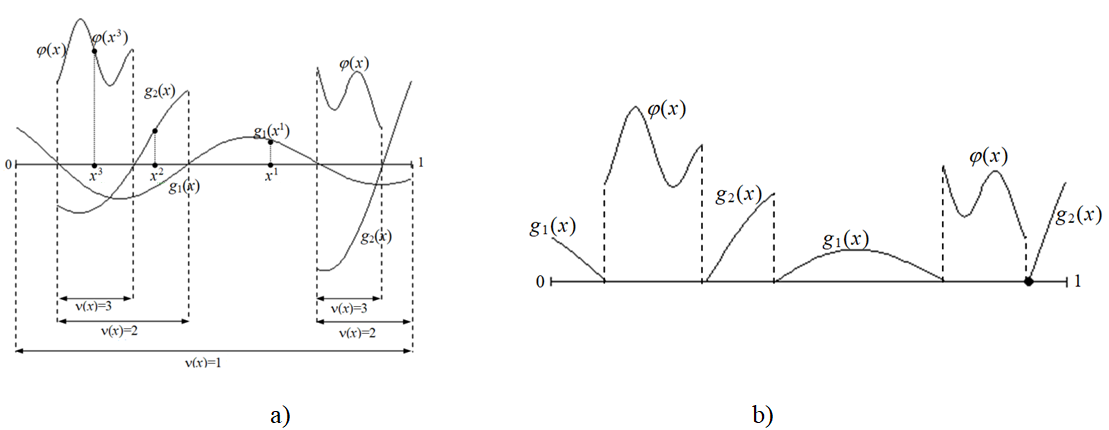
\includegraphics[width=\linewidth]{fig1}
  \caption{An integrated function for the problem (\ref{eq:13}) using a sequential constraint calculation scheme: a) the function $F(x)$ from (\ref{eq:16}), b) the function $\Phi(x)$ from (\ref{eq:17})}
  \label{fig:1}
\end{figure}

The function $F(x)$ consists of separate fragments of the constraints $g_i(x) \leq 0$, $1 \leq i \leq m$, and the minimized function $\varphi(x)$. For the homogeneity of the components, the function $F(x)$ is then converted to the form 
\begin{equation}\label{eq:17}
\Phi (x) = 
 \begin{cases}
   g_\nu(x) / H_\nu, & \nu < M, \\
   (g_M(x)-z^*_M) / H_M, & \nu = M,
 \end{cases}
\end{equation}
where $M$ is the constraint number for which there are no feasible points (the maximum value of the index is $\nu(x)$), $z^*_M$ is the value of the minimum constraint violation $g_M(x)$\footnote{If $M=m+1$, then $z_M^*$ is the minimum value of the function $\varphi(x)$.}, and $H_\nu$, $1\leq \nu \leq M$, are the H\"older constants from (\ref{eq:11}). As a rule, these values are a priori unknown, but when performing calculations, instead of these values, their adaptive estimates obtained in the process of calculations can be applied. For this, the search information $A_k$ from (\ref{eq:12}) should be expanded with data
\begin{equation}\label{eq:18}
A_k=\{(x_i, z_i, \nu_i, y(x_i), f_i=f( y(x_i))): 1 \leq i \leq k \},
\end{equation}
where $z_i= \Phi(x_i)$, $1 \leq i \leq k$. Then estimates of the required values can be determined as follows
\begin{equation}\label{eq:19}
M^k= \max{\{\nu=\nu(x_i), 1\leq i \leq k \}},
\end{equation}

\begin{equation}\label{eq:20}
z^k_\nu = 
 \begin{cases}
   0, & \nu < M, \\
   \min{\{g_\nu(x_i):\nu=\nu(x_i), 1\leq i \leq k \}}, & \nu = M,
 \end{cases}
\end{equation}

\begin{equation}\label{eq:21}
h^k_l=\max{\{|z_i-z_j|/\sqrt[N]{x_i-x_j},\nu_i=\nu_j=l,i>j,1\leq l\leq M^k\}}
\end{equation}

If $h_l^k$ in (\ref{eq:21}) turns out to be indefinite or equal to zero, then $h_l^k=1$ is taken. For the initial values of these quantities, $M^0 = H_l^0=1$, $z_l^0=0$, $1 \leq i \leq m+1$ can be taken.

The general computational scheme of the global search algorithm for multiextremal optimization problems with nonlinear constraints \footnote{This method is also known as the index method -- see \cite{c18}.} (AGCS) is as follows \cite{c18}.

The first trial is carried out at an arbitrary internal point $x^1\in (0,1)$. The calculation results are constantly added to the set $A_k$ from (\ref{eq:12}); in addition, into $A_k$ are also added the points $x_0=0$ and $x_{k+1}=1$ (the values $z_0$ and $z_{k+1}$ are not defined and not used) for the convenience of subsequent formulations. The choice of the point $x^{k+1}$, $k\geq 1$, of any next trial is determined by the following rules.

\textit{Rule 1.} For each interval $(x_{i-1},x_i)$, $1 \leq i \leq k+1$, in the set $A_k$ calculate the characteristic $R(i)$, where
\begin{equation}\label{eq:22}
\begin{matrix}
R(i) = 
 \begin{cases}
   \rho_i + \frac{(z_i-z_{i-1})^2}{r^2_\nu h^2_\nu \rho_i} - 2 \frac{z_i+z_{i-1}-2z^*_\nu}{r_\nu h_\nu}, & \nu=\nu(x_{i-1})=\nu(x_i), \\
   2 \rho_i - 4\frac{z_i-z^*_\nu}{r_\nu h_\nu}, & \nu=\nu(x_{i-1})<\nu(x_i), \\
2 \rho_i - 4\frac{z_{i-1}-z^*_\nu}{r_\nu h_\nu}, & \nu=\nu(x_{i-1})>\nu(x_i), 
 \end{cases} \\
\rho_j = \sqrt[N]{x_i-x_{i-1}}, 1\leq j\leq k+1.
\end{matrix}
\end{equation}

The constants $r_\nu>1$, $1\leq \nu \leq m+1$, are the parameters of the algorithm. The products $r_\nu h_\nu$ are used as an estimate of the H\"older constants $H_\nu$, $1\leq \nu \leq m+1$ from (\ref{eq:11}).

\textit{Rule 2.} Determine the interval $(x_{t-1},x_t)$ that corresponds to the maximum characteristic
\begin{equation}\label{eq:23}
R(t) = \max{\{R(i):1 \leq i \leq k+1\}}.
\end{equation}

\textit{Rule 3.} Execute a new trial at the point $x^{k+1} \in (x_{t-1},x_t)$, determined in accordance with the expression
\begin{equation}\label{eq:24}
x^{k+1} = 
 \begin{cases}
   \frac{x_t+x_{t-1}}{2}, & \nu(x_{t-1}) \neq \nu(x_t), \\
   \frac{x_t+x_{t-1}}{2} + sign(z_t - z_{t-1}) \frac{1}{2r_\nu}[ \frac{|z_t - z_{t-1}|}{h_\nu}^N ], & \nu = \nu(x_{t-1}) = \nu(x_t).
 \end{cases}
\end{equation}

Iterations of the algorithm are terminated if the stop condition is satisfied
\begin{equation}\label{eq:25}
\rho_t\leq \varepsilon,
\end{equation}
where $t$ from (\ref{eq:23}) and $\varepsilon > 0$ is the given accuracy.

Results of using the AGCS algorithm to solve the test problem from Fig.~\ref{fig:1} with the parameters $r_1=r_2=r_3=2$ and $\varepsilon=10^{-5}$ are shown in Fig. \ref{fig:2}.  The coordinates of the trial points performed by the algorithm in the process of solving the problem are marked in Fig. \ref{fig:1} by three rows of vertical strokes. The strokes in the upper row correspond to points with a unit index, the second row to points whose indices equal to 2; the points marked with strokes in the bottom row belong to the feasible domain. The coordinates of trials performed at close points are marked with a dark rectangle. In total, the value of the first constraint was computed 147 times, the value of the second constraint -- 84 times, and the value of the minimized function was calculated only 35 times.

\begin{figure}
  \centering
  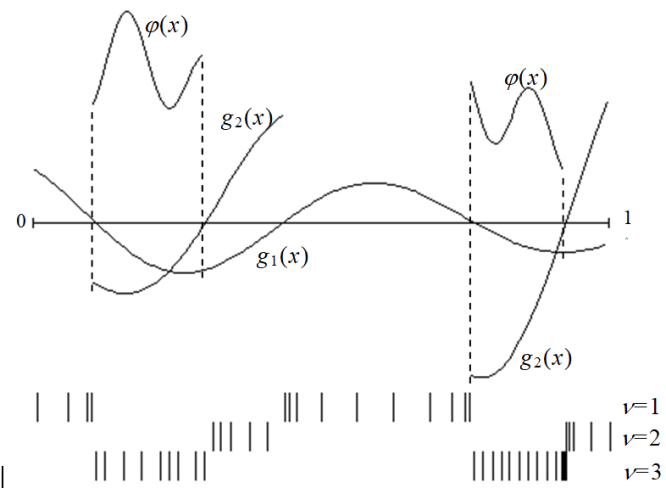
\includegraphics[width=0.6\linewidth]{fig2}
  \caption{Results of using the AGCS algorithm to solve the test problem}
  \label{fig:2}
\end{figure}

Various modifications of this algorithm and the corresponding theory of convergence are presented in \cite{c18}. For instance, the following theorem is valid.

\begin{theorem}
If the AGCS algorithm is used to solve problem (\ref{eq:13}), and the following conditions are satisfied:
\begin{enumerate}
	\item the functions $g_j$, $1 \leq j \leq m+1$,  satisfy the H\"older condition of (\ref{eq:11}) with the constants $H_j$, $1 \leq j \leq m+1$,
	\item for the quantities $h_\nu$ from (\ref{eq:21}), starting from a certain step, the inequalities are valid
\begin{equation*}
r_\nu h_\nu>2H_\nu, 1\leq \nu \leq m+1,
\end{equation*}
\end{enumerate}
then the set of limit points of the sequence $\{x^k\}$, generated by the algorithm coincides with the set of global minimum points of the problem (\ref{eq:13}) with $\varepsilon=0$ in the stop condition (\ref{eq:25}).
\end{theorem}

\subsection{Acceleration of computations based on the re-use of search information}

As noted earlier, the MCOlex problem at each stage of the successive concessions method (\ref{eq:7}) is a global optimization problem with nonlinear constraints (\ref{eq:13}). Generally, the solution to such problems must start at the beginning, and multiple solutions of such global optimization problems may require extensive calculations. However, the presence of search information $A_k$ from (\ref{eq:18}) allows us to bring the results of previous calculations to the values of any next solved optimization problem in the scheme (\ref{eq:7}) without any time-consuming calculations of the values of the criteria $f_i (y)$, $1 \leq j \leq s$,  of the initial problem (\ref{eq:1}) \cite{c30,c31}. This re-use of search information, to find the next efficient decision, reduces the amount of computations needed to solve each next optimization problem to just a few iterations; see Section \ref{sec:4} for the results of computational experiments.

Moreover, using search information $A_k$ allows to reduce the multistage solution of the MCO problem in accordance with the scheme (\ref{eq:7}) to the solution of the only global optimization problem in the last stage of the scheme (\ref{eq:7}), namely 
\begin{equation}\label{eq:26}
P_{\delta lex} (f,\delta,D)=Arg \min_{y\in D}{f_s(y)}, f_j(y)\leq f_j^*+\delta_j, 1 \leq j < s,
\end{equation}
where for the unknown a priori values $f_j^*$, $1 \leq j < s$, can be used the estimates $z_j^k$, $1 \leq j < s$, from (\ref{eq:20}) obtained from the search information $A_k$,  and for the constants $\delta_j$, $1 \leq j<s$, we can use the values normalized to the range of the constraints' values, that is
\begin{equation}\label{eq:27}
	\begin{matrix}
	\delta_j=z_j^k+\theta_j (g_j^k-z_j^k ),\; 0\leq \theta_j\leq 1, \; 1 \leq j < s,\\
	g_j^k= \max{\{ g_j (x_i ) : \nu(x_i)=j,\; 1\leq i\leq k \}}.
	\end{matrix}
\end{equation}

The applicability of such a one-step scheme (\ref{eq:26})--(\ref{eq:27}) instead of the scheme (\ref{eq:7}) is computationally evaluated in Section \ref{sec:4}.

With a complete scheme for calculating criteria values, i.e. when at the iteration points $x_i$, $1 \leq i \leq k$,  the values of all criteria $f_j (x_i)$, $1 \leq j \leq s$, $1 \leq i \leq k$, are calculated, the effect of using the search information $A_k$ can be even more significant. In this case, the search information can also be used when changing the values of the concessions $\delta_j$, $1 \leq j < s$, and thus, the solution of the next problem from the $\mathbb{P}_t$ family (\ref{eq:8}) can be carried out repeatedly using the results of all previously performed calculations. Results of computational experiments (see Section \ref{sec:4}), demonstrate that the volume of computations performed, based on reusing search information, is reduced by a factor of no less than 6.

The AGCS algorithm, supplemented by the ability to use search information to solve multiple MCOlex  problems, will be referred to below as the global search algorithm for multistage solutions of a set of multiextremal optimization problems with nonlinear constraints (MAGCS).

\section{Results of computational experiments}
\label{sec:4}

The computational experiments were carried out on the Lobachevsky supercomputer at Nizhny Novgorod State University (the operating system CentOS 6.4, the management system SLURM). A supercomputer node has 2 Intel Sandy Bridge E5-2660 2.2 GHz, 64 Gb RAM processors. Each CPU is 8-core; that is, there are 16 CPU cores available on the node. The Intel C++ 14.0.2 compiler was used to obtain an executable program code. The numerical experiments were performed using the Globalizer system \cite{c32}.

The global optimization algorithms used within the framework of the proposed approach have proven to be efficient in the process of conducting test computational experiments and have been widely used in solving practical optimization problems (see, e. g., \cite{c33,c34}). The results of computational experiments in solving multicriteria optimization problems are given below.

In the first series of computational experiments, the developed MAGCS algorithm was compared with several multicriteria optimization algorithms. To make a comparison, we used the test two-criteria problem proposed in \cite{c35}:
\begin{equation}\label{eq:28}
f_1 (y)=(y_1-1) y_2^2+1,f_2 (y)=y_2, 0\leq y_1,y_2 \leq 1.
\end{equation}


Solving the MCO problem was understood to mean constructing a numerical approximation of the Pareto domain. To assess the quality of the approximation, the completeness and uniformity of the Pareto domain coverage were compared, using the following two indicators \cite{c35,c36}:
\begin{itemize}
	\item 	The hypervolume index (HV). This indicator characterizes the approximation of the Pareto domain in terms of completeness; a higher value corresponds to a more complete coverage of the Pareto domain.
	\item The distribution uniformity index (DU). This indicator characterizes the uniformity of Pareto domain coverage; a lower value corresponds to a more uniform coverage of the Pareto domain.
\end{itemize}
	
In the framework of this experiment, five multicriteria optimization algorithms were compared: the Monte-Carlo (MC) method, the genetic algorithm SEMO from the PISA library \cite{c9,c36}, the Non-uniform coverage (NUC) method \cite{c35}, the bi-objective Lipschitz optimization (BLO) method \cite{c36}, and the MAGCS algorithm proposed in this paper. The results of solving problem (\ref{eq:28}) for all these methods (except for MAGCS) were obtained in \cite{c36}.

For MAGCS, 50 problems (\ref{eq:26}) were solved for different values $\theta_j$, $1 \leq j<s$, uniformly distributed in the interval [0,1]. The accuracy from (\ref{eq:25}) $\varepsilon=0.05$ and the reliability from (\ref{eq:22}) $r=3.0$ were used. The results of the executed experiments are presented in Table \ref{tab:1}.

\begin{table}[ht]
\centering
\caption{The numerical results of solving the multicriteria optimization problems from (\ref{eq:28})}
\label{tab:1}
\begin{tabular}{cccccc}
\hline
Method                                                                                     & MC    & SEMO  & NUC   & BLO   & \textbf{MAGCS} \\ \hline
Number of executed iterations                                                              & 500   & 500   & 515   & 498   & \textbf{273}   \\
\begin{tabular}[c]{@{}c@{}}Number of points in \\ Pareto domain approximation\end{tabular} & 67    & 104   & 29    & 68    & \textbf{80}    \\
HV index                                                                                   & 0.300 & 0.312 & 0.306 & 0.308 & \textbf{0.314} \\
DU index                                                                                   & 1.277 & 1.116 & 0.210 & 0.175 & \textbf{0.096} \\ \hline
\end{tabular}
\end{table}

The results from the executed experiments demonstrate that the MAGCS algorithm has a significant advantage in comparison with the considered multicriteria optimization methods, even when solving relatively simple MCO problems.

In the second series of computational experiments, two-criteria two-dimensional MCO problems were solved. Multiextremal functions obtained using the GKLS generator \cite{c37} served as the criteria for the problem. During the experiments, 100 multicriteria problems of this class were solved. In each problem, Pareto-optimal decisions were searched for 50 different values of $\theta_j$, $1\leq j < s$, uniformly distributed in the interval [0,1]; (that is, 5,000 global optimization problems were solved). The results obtained were averaged over the number of MCO problems solved.

In the computational experiments, calculations are terminated when the required accuracy was achieved. When the process was terminated, the solution was evaluated for correctness. As a means of control, we compared the solution points found by MAGCS and the points calculated from the Pareto boundary, taking into account the selected values of $\theta_j$, $1 \leq j < s$. The method parameters were set as follows: the accuracy $\varepsilon = 0.02$ and the reliability $r_1=r_2=5.6$. Results of the computational experiments are presented in Table 2.

In Table 2, the first and fifth columns indicate the average number of iterations executed by the MAGCS algorithm for solving the MCOlex problems. The second and sixth columns contain the percentage of completed problems. The third, fourth, seventh and eighth columns show the values of HV and DU indicators. The last column gives values showing the reduction in the number of global search iterations that were executed when solving the MCOlex problems, by reusing search information.


\begin{table}[ht]
\centering
\caption{Results of the series of experiments to solve two-dimensional two-criteria MCO problems}
\label{tab:2}
\resizebox{\columnwidth}{!}{
\begin{tabular}{ccccccccccc}
\hline
\multicolumn{10}{c}{Search information}                                    & Reduction \\ \cline{1-9}
\multicolumn{4}{c}{not used}         & & \multicolumn{4}{c}{used}             &  & in \\ \cline{1-4} \cline{6-9}
Method     & Problem & Avg   & Avg   & & Method     & Problem & Avg   & Avg   &  & iteration    \\
iter.      & solved  & HV    & DU    & & iter.      & solved  & HV    & DU    &  & number       \\ \cline{1-4} \cline{6-9} \cline{11-11}
41 710.1   & 98.0\%  & 33.43 & 0.173 & & 2 407.41   & 99.3\%  & 33.34 & 0.224 &  & 17.3         \\ \hline
\end{tabular}
}
\end{table}


Results obtained from these experiments show that the re-use of search information can reduce the amount of calculations by 17.3 times without expending additional computational resources, and according to the average HV and DU indicators, the quality of the Pareto domain remains on average at the same level.

In the third series of computational experiments, the two-criteria four-dimensional MCO problems were solved. As in the second series of computational experiments, 100 multicriteria problems were solved. In each problem, the Pareto-optimal decisions were calculated for 50 different values of $\theta_j$, $1 \leq j <s$, uniformly distributed in the interval $[0,1]$. The criteria of the MCO problems being solved were determined using the GKLS generator \cite{c37}. The method parameters were set as follows: the accuracy $\varepsilon = 0.025$ and the reliability $r_1=r_2=5.6$. The results of computational experiments are presented in Table 3.


\begin{table}[ht]
\centering
\caption{Results of the series of experiments to solve two-criteria four-dimensional MCO}
\label{tab:3}
\resizebox{\columnwidth}{!}{
\begin{tabular}{ccccccccccc}
\hline
\multicolumn{10}{c}{Search information}                                        & Reduction   \\ \cline{1-9}
\multicolumn{4}{c}{not used}       & & \multicolumn{4}{c}{used}                & &  in       \\ \cline{1-4} \cline{6-9}
Method      & Problem & Avg   & Avg   & & Method     & Problem & Avg   & Avg   & & iteration \\
iter.       & solved  & HV    & DU    & & iter.      & solved  & HV    & DU    & & number    \\ \cline{1-4} \cline{6-9} \cline{11-11}
4 536 377.9 & 83.0\%  & 30.67 & 0.335 & & 709 014.9  & 94.5\%  & 30.46 & 0.405 & & 6.4       \\ \hline
\end{tabular}
}
\end{table}


Results from the executed experiments show that with increased dimensions of MCO problems to be solved and a corresponding increase in the volume of calculations, the efficiency of the MAGCS algorithm remains at a high level;  its use has efficiently reduced the number of the executed iterations by 6.4 times.



\section{Conclusion}
\label{sec:5}

This paper proposes a new approach for solving computationally expensive lexicographic multicriteria optimization problems (MCOlex), in which the efficiency criteria can be multiextremal, and calculating the criteria values may require a large amount of computation. A key feature of this class of problems is the ability, during the computation process, to alter the ordering of efficiency criteria in terms of importance, which in turn necessitates a multistage solution for MCOlex problems.

Overcoming the enormous computational complexity of addressing the formulated new class of MCOlex problems is ensured by solving a sequence of global optimization problems with nonlinear constraints using efficient information-statistical methods of global optimization by using an original index constraint accounting scheme instead of the commonly used penalty functions. A core element in this approach is the ability to use all the search information obtained in the computation process, utilizing the multistage solution of MCOlex problems. Starting to solve each new stage of the solution, this search information allows us to incorporate the previously calculated values of efficiency criteria into the values of the next scalar problem of multiextremal optimization. The search information retrieved becomes part of the current optimization state and through optimization methods, results in adaptive planning of the iterations to run the global search. 

Results of computational experiments demonstrate that this approach can significantly reduce the computational complexity of multistage MCOlex problem solving.

In conclusion, it must be noted that the approach described here is promising, and requires further research. Importantly, it is necessary to continue carrying out computational experiments to solve multicriteria optimization problems with a larger number of efficiency criteria and for greater dimensions in the optimization problems to be solved. It is also necessary to evaluate the possibility of parallel computing using high-performance supercomputer systems.


% Non-BibTeX users please use
\begin{thebibliography}{}
%
% and use \bibitem to create references. Consult the Instructions
% for authors for reference list style.
%

\bibitem{c1} Miettinen K.: Nonlinear Multiobjective Optimization. Springer. (1999)
\bibitem{c2} Ehrgott, M.: Multicriteria Optimization. Springer. (2nd ed., 2010)
\bibitem{c3} Collette, Y., Siarry, P.: Multiobjective Optimization: Principles and Case Studies (Decision Engineering). Springer. (2011)
\bibitem{c4} Marler, R.T., Arora, J.S.: Multi-Objective Optimization: Concepts and Methods for Engineering. VDM Verlag. (2009)
\bibitem{c5} Pardalos, P.M., {\v Z}ilinskas, A., {\v Z}ilinskas, J.: Non-Convex Multi-Objective Optimization. Springer. (2017)
\bibitem{c6} Marler, R. T., Arora, J. S.: Survey of multi-objective optimization methods for engineering. Struct. Multidisciplinary Optimization 26, pp. 369--395 (2004)
\bibitem{c7} Figueira,J., Greco, S., Ehrgott, M., editors.: Multiple criteria decision analysis: State of the art surveys. Springer, New York (NY). (2005)
\bibitem{c8} Zavadskas, E. K., Turskis, Z., Kildien\.e, S.: State of art surveys of overviews on MCDM/MADM methods. Technological and Economic Development of Economy, 20, pp. 165--179 (2014)
\bibitem{c9} Hillermeier, C., Jahn, J.: Multiobjective optimization: survey of methods and industrial applications. Surv. Math. Ind. 11, pp. 1--42 (2005)
\bibitem{c10} Branke, J., Deb, K., Miettinen, K., Slowinski, R., editors.: Multi-Objective Optimization—Interactive and Evolutionary Approaches. Springer, Berlin. (2008)
\bibitem{c11} Deb, K.: Multi-Objective Optimization using Evolutionary Algorithms. Wiley, Chichester. (2001)
\bibitem{c12} Yang, X.-S.: Nature-inspired metaheuristic algorithms. Luniver Press, Frome. (2008) 
\bibitem{c13} Tan, K.C., Khor, E.F., Lee, T.H.: Multi-objective Evolutionary Algorithms and Applications. Springer-Verlag, London. (2005)
\bibitem{c14} Eichfelder, G.: Scalarizations for adaptively solving multi-objective optimization problems. Comput. Optim. Appl. 44, pp. 249--273 (2009)
\bibitem{c15} Jones, D.R.: A taxonomy of global optimization methods based on response surfaces. J. Glob. Optim. 21, pp. 345--383 (2001)
\bibitem{c16} Voutchkov, I., Keane, A.: Multi-objective optimization using surrogates. Comput. Intell. Optim. Adapt. Learn. Optim. 7, pp. 155--175 (2010)
\bibitem{c17} Strongin, R.G.: Numerical methods in multiextremal problems: information-statistical algorithms. Nauka, Moscow. (1978, in Russian) 
\bibitem{c18} Strongin, R., Sergeyev, Ya.: Global optimization with non-convex constraints. Sequential and parallel algorithms. Kluwer Academic Publishers, Dordrecht. (2nd ed. 2013, 3rd ed. 2014).
\bibitem{c19} T\"orn, A., {\v Z}ilinskas, A.: Global Optimization. Lecture Notes in Computer Science, 350. Springer-Verlag, Berlin. (1989)
\bibitem{c20} Horst, R., Tuy, H.: Global Optimization: Deterministic Approaches. Springer-Verlag, Berlin. (1990)
\bibitem{c21} Zhigljavsky, A.A.: Theory of Global Random Search. Kluwer Academic Publishers, Dordrecht. (1991)
\bibitem{c22} Pint\'er, J.D.: Global optimization in Action (continuous and Lipschitz optimization: algorithms, implementations and applications). Kluwer Academic Publishers, Dortrecht. (1996)
\bibitem{c23} Sergeyev Y.D., Strongin R.G., Lera D.: Introduction to global optimization exploiting space-filling curves. Springer. (2013)
\bibitem{c24} Locatelli, M., Schoen, F.: Global Optimization: Theory, Algorithms, and Applications. SIAM. (2013)
\bibitem{c25} Floudas, C.A., Pardalos, M.P.: Recent Advances in Global Optimization. Princeton University Press. (2016)
\bibitem{c26} Lera D., Sergeyev Ya.D.: Deterministic global optimization using space-filling curves and multiple estimates of Lipschitz and Holder constants, Communications in Nonlinear Science and Numerical Simulation, 23. pp. 328--342 (2015)
\bibitem{c27} Gergel, V.: A Unified Approach to Use of Coprocessors of Various Types for Solving Global Optimization Problems. 2nd International Conference on Mathematics and Computers in Sciences and in Industry. pp. 13--18 (2015). DOI: 10.1109/MCSI.2015.18
\bibitem{c28} Arora, R.K.: Optimization: Algorithms and Applications. CRC Press. (2015)
\bibitem{c29} Bazaraa, M.S., Sherali, H.D., Shetty, C. M.: Nonlinear Programming: Theory and Algorithms, John Wiley and Sons. (2006)
\bibitem{c30} Gergel, V.P., Kozinov, E.A.: Accelerating multicriterial optimization by the intensive exploitation of accumulated search data. In: AIP Conference Proceedings, 1776. pp. 090003 (2016). DOI: 10.1063/1.4965367
\bibitem{c31} Gergel, V.P., Kozinov, E.A.: Efficient multicriterial optimization based on intensive reuse of search information.  J. Glob. Optim., 71(1). pp. 73--90 (2018). DOI: 10.1007/s10898-018-0624-3
\bibitem{c32} Sysoyev, A., Barkalov, K., Gergel, V.: Globalizer: A novel supercomputer software system for solving time-consuming global optimization problems. Numerical Algebra, Control and Optimization 8(1), pp. 47--62 (2018)
\bibitem{c33} Kvasov D.E., Sergeyev Y.D.: Deterministic approaches for solving practical black-box global optimization problems. Advances in Engineering Software, 80, pp.58--66 (2015)
\bibitem{c34} Modorskii, V., Gaynutdinova, D., Gergel, V., Barkalov, K.: Optimization in design of scientfic products for purposes of cavitation problems. AIP Conference Proceedings, 1738. (2016)
\bibitem{c35} Evtushenko, Yu.G., Posypkin, M.A.: A deterministic algorithm for global multi-objective optimization. Optimization Methods \& Software, 29(5), pp. 1005--1019 (2014)
\bibitem{c36} {\v Z}ilinskas, A., {\v Z}ilinskas, J.: Adaptation of a one-step worst-case optimal univariate algorithm of bi-objective Lipschitz optimization to multidimensional problems. Commun Nonlinear Sci Numer Simulat, 21, pp. 89--98 (2015)
\bibitem{c37} Gaviano, M., Kvasov, D.E, Lera, D., and Sergeyev, Ya.D.: Software for generation of classes of test functions with known local and global minima for global optimization. ACM Transactions on Mathematical Software 29(4). pp. 469--480 (2003)

\end{thebibliography}

\end{document}
% end of file template.tex

